\section{ОХРАНА ТРУДА И БЕЗОПАСНОСТИ В ЧРЕЗВЫЧАЙНЫХ СИТУАЦИЯХ}

\subsection{Анализ условий труда в помещении офиса}

Помещение офиса находиться на первом этаже четырехэтажного железобетонного здания,
содержит одно рабочее место, которое включает: 
два ПК в комплектации: системный блок, жидкокристаллический экран, мышь, клавиатура.

Размеры помещения: длина -- 4 м, ширина -- 3 м, высота -- 2.5 м. Нормой, в соответствии с ДСанПiН 3.3.2-007-98, 
является площадь на одно рабочее место не менее 6,0 кв. м, объём -- не менее 20,0 куб. м, которая в данном случае
соблюдена. Помещение офиса включает 1 рабочее место площадью 12 кв. м, объёмом 30 куб. м.

Проведем анализ системы <<Человек-Машина-Среда>> (Ч-М-С), структурная схема которой показана на рисунке 
\ref{fig:hme},
а направление связей приведено в таблице \ref{tab:hme}. Все элементы условно разделены на функциональные части:

\begin{description}
    \item [\(\text{Ч}_1\)] --- функциональная задача элемента -- управление <<машиной>> для получения предмета труда;
    \item [\(\text{Ч}_2\)] --- биологический обьект, непосредственно влияющий на среду за счет влаго-, тепло- и энерговыделения;
    \item [\(\text{Ч}_3\)] --- физиологическое состояние человека с учетом факторов, влияющих на него в процессе работы;
    \item [\(\text{Ч}_1\)] --- выполняет основную технологическую функцию;
    \item [\(\text{Ч}_2\)] --- выполняет функцию аварийной защиты;
    \item [\(\text{Ч}_3\)] --- служит источником вредных влияний на человека и ОС;
    \item [\(\text{Среда}\)] --- внутренняя среда помещения: освещение, микроклимат и т.д.
    \item [\(\text{Предмет труда}\)] --- результат профессиональной деятельности человека.
\end{description}

\begin{figure}[!ht]
    \centering
    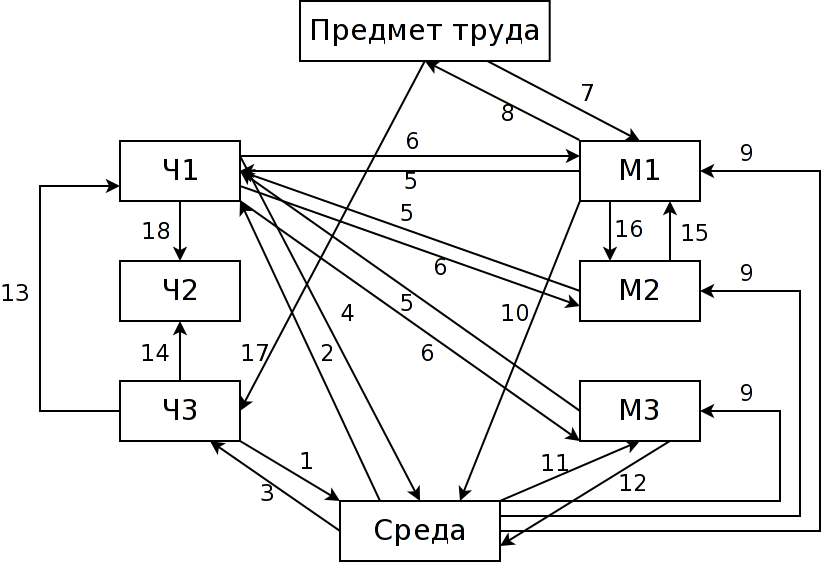
\includegraphics[scale=0.4]{graphics/hme.png}
    \caption{Система ``Человек-Машина-Среда''}
    \label{fig:hme}
\end{figure}

\begin{center}
   \begin{longtable}{|p{1cm}|p{3cm}|p{12cm}|}
       \caption{Направление связей в системе <<Человек-Машина-Среда>>} \label{tab:hme} \\ \hline
       № & Связь & Содержание \\
       \endfirsthead

       \caption{Направление связей в системе <<Человек-Машина-Среда>> (продолжение)} \label{tab:hme} \\ \hline
       № & Связь & Содержание \\
       \endhead

       \hline
        1 & \(\text{Ч}_3-\text{С}\)   & Влияние оператора как биологического объекта на среду \\
       \hline
        2 & \(\text{С}-\text{Ч}_1\)   & Влияние окружающей среды на качество работы оператора \\
       \hline
        3 & \(\text{С}-\text{Ч}_3\)   & Влияние окружающей среды на состояние организма оператора \\
       \hline
        4 & \(\text{Ч}_1-\text{С}\)   & Информация про состояние среды, обрабатываемая оператором \\
       \hline
        5 & \(\text{М}_1, \ \text{М}_2, \ \text{М}_3-\text{Ч}_1\) & Информация про состояние ЭВМ обрабатываемая оператором \\
       \hline
        6 & \(\text{Ч}_1-\text{М}_1, \ \text{М}_2, \ \text{М}_3\) & Влияние оператора на управление ЭВМ и ее настройку \\
       \hline
        7 & \(\text{ПТ}-\text{М}_1\)  & Информация про объект труда, получаемая ЭВМ \\
       \hline
        8 & \(\text{М}_1-\text{ПТ}\)  & Влияние ЭВМ на объект труда \\
       \hline
        9 & \(\text{С}-\text{М}_1, \ \text{М}_2, \ \text{М}_3\)  & Влияние окружающей среды на работу ЭВМ \\
       \hline
       10 & \(\text{М}_1-\text{С}\)   & Влияние ЭВМ на среду \\
       \hline
       11 & \(\text{С}-\text{М}_3\)   & Информация про окружающую среду, получаемая ЭВМ \\
       \hline
       12 & \(\text{М}_3-\text{С} \)  & Целенаправленное влияние ЭВМ на среду \\
       \hline
       13 & \(\text{Ч}_3-\text{Ч}_1\) & Влияние состояние организма оператора на качество его работы \\
       \hline
       14 & \(\text{Ч}_3-\text{Ч}_2\) & Влияние физиологического состояния оператора на степень интенсивности обмена веществ
                                        между организмом и средой, и энерговыделение оператора \\
       \hline
       15 & \(\text{М}_2-\text{М}_1\) & Аварийное управляющее влияние \\
       \hline
       16 & \(\text{М}_1-\text{М}_2\) & Информация, необходимая для создания аварийных управляющих влияний \\
       \hline
       17 & \(\text{ПТ}-\text{Ч}_2 \) & Влияние предмета труда на психологическое состояние человека \\
       \hline
       18 & \(\text{Ч}_1-\text{Ч}_2\) & Влияние интенсивности работы программиста на физиологические функции \\
       \hline
   \end{longtable}
\end{center}

В помещении офиса, согласно ГОСТ 12.0.003-74, имеют место следующие опасные и вредные производственные факторы:
физические, психофизиологические. Химические и биологические факторы в данном помещении отсутствуют. 

К физическим факторам относятся: повышенный уровень шума на рабочем месте;
повышенное значение напряжения в электрической цепи, замыкание которой может
произойти через тело человека; повышенная или пониженная температура;
недостаток естественного света; недостаточная освещенность рабочей зоны. 

К психофизиологическим относятся: физические статические перегрузки; умственное перенапряжение; 
перенапряжение зрительных анализаторов; эмоциональные перегрузки.

Оценка факторов производственной среды и трудового процесса приведена в таблице \ref{tab:factors}.	

{\normalsize
\begin{longtable}[c]{|p{7cm}|p{2cm}|p{2cm}|p{0.5cm}|p{0.5cm}|p{0.5cm}|p{2cm}|}
    \caption{Оценка факторов производственной среды и трудового процесса} \label{tab:factors} \\

    \hline
\multirow{2}{*}{Фактор} & \multicolumn{2}{c|}{Значение фактора} & \multicolumn{3}{c|}{3 класс} & Действие, \\
\cline{2-6} & Норма & Факт & 1 ст. & 2 ст. & 3 ст. & \% смены \\ \hline
        \endfirsthead

        \caption{Оценка факторов производственной среды и трудового процесса (продолжение)} \label{tab:map} \\

        \hline
\multirow{2}{*}{Фактор} & \multicolumn{2}{c|}{Значение фактора} & \multicolumn{3}{c|}{3 класс} & Действие, \\
\cline{2-6} & Норма & Факт & 1 ст. & 2 ст. & 3 ст. & \% смены \\ \hline
    \endhead

    Шум, ДБа & \(\le 50\) & 50 & + & -- & -- & \\
    \hline
    Неионизирующее излучение: & & & & & & \\
    а) промышленные частоты, \(\frac{\text{В}}{\text{м}}\)      & \(\le 25\)  & 1,2 & -- & -- & -- & 100 \\
    б) радиотехнический диапазон, \(\frac{\text{В}}{\text{м}}\) & \(\le 2,5\) & 1,0 & -- & -- & -- & 100 \\
    \hline
    Рентгеновское излучение, \(\frac{\text{мкР}}{\text{ч}}\)    & \(\le 100\) & 22          & -- & -- & -- & 80 \\
    \hline
    Микроклимат:                                                  &             &             &     &     &     &     \\
    а) температура воздуха, \(^{\circ}\mathrm{C}\)                & 22 -- 24    & 23          & --  & --  & --  & 100 \\
    б) скорость движения воздуха, \(\frac{\text{м}}{\text{с}}\)   & \(\le 0,1\) & \(\le 0,1\) & --  & --  & --  & 100 \\
    в) относительная влажность, \%                                & 40 -- 60    & 61          & --  & --  & --  & 100 \\
    \hline
    Освещение:            &               &     &     &     &     &    \\
    а) естественное, КЕО  & \(\ge 1,5\%\) & 4\% & --  & --  & --  & 70 \\
    б) искусственное, лк  & 300--500      & 250 &  +  & --  & --  & 30 \\
    \hline
    Тяжесть труда:         &               &     &     &     &     &    \\
    а) мелкие стереотипные
       движения, кол-во за
       смену                          & \(\le 40000\) & 45000 & +   & -- & -- & 100 \\
    б) рабочая поза, \%               & \(\le 25\)    & 20    & --  & -- & -- & 20  \\
    в) перемещение в пространстве, км & \(\le 10\)    & 1     & --  & -- & -- & 5   \\
    \hline
    Напряжённость труда: время наблюдения
    за ходом производственного процесса, ч & \(2 \div 3\) & 4 & + & -- & -- & 90 \\
    \hline
    Сменность: & 2-х сменная работа без ночной смены & 2-х сменная работа без ночной смены & -- & -- & -- & -- \\
    \hline
    Количество факторов: &  &  & 3 & -- & -- & \\
    \hline
\end{longtable}
}
По результатам гигиенической оценки условий труда было выявлено, что условия и характер труда относятся
к III классу 1 степени вредности, и не соответствуют требованиям гигиенической классификации.
Так как доминирующим вредным фактором является недостаточная освещенность рабочей зоны, то для снижения
его вредного влияния произведен выбор и расчет системы искусственного освещения помещения офиса. 

\subsection{Промышленная безопасность в помещении офиса}

По степени опасности поражения электрическим током, помещение офиса относится к классу помещений без повышенной
опасности согласно НПАОП 40.1-1.21-98, так как исключена возможность одновременного прикосновения человека к корпусам
электроприборов и к заземленным металлическим конструкциям здания.

Электроснабжение оборудования осуществляется от трехфазной четырехпроводной сети с глухозаземленной нейтралью,
ток переменный, напряжение 380/220 В. В соответствии с требованиями НПАОП 40.1-1.32-01 для электрооборудования
переменного тока напряжением до 1000 В используется зануление для устранения опасности поражения людей электрическим
током при пробое на корпус. 

Сечение нулевого защитного проводника, выполненного из медного провода, такое же, как и сечение фазного провода.
Для обеспечения работы зануления обеспечена непрерывность цепи от каждого корпуса ПЭВМ до нейтрали источника.
Кроме того нулевой защитный проводник подлежит повторному заземлению, что снижает потенциал занулённых корпусов
и напряжение прикосновения в случае обрыва цепи зануления. Сопротивление первичного заземлителя нейтрали не более
4 Ом при напряжении сети 380\slash220 В, сопротивление изоляции сети не менее 0,5 МОм, сопротивление одиночного повторного
заземления нулевого провода не более 30 Ом согласно требованиям НПАОП 40.1-1.32-01. 

Электросеть розеток для питания ПЭВМ проложена под съемным полом в гибких металлических рукавах.

Согласно НПАОП 0.00-4.12-05 проводится вводный, первичный на рабочем месте, повторный, а при необходимости -- 
внеплановый и целевой инструктажи.

\subsection{Производственная санитария в офисном помещении}

Так как работа производится сидя и не требует физического напряжения (энергозатраты организма до120 ккал\slashч),
она относится к работам категорий I а согласно ДСН 3.3.6-042-99. Оптимальные и допустимые параметры микроклимата,
согласно ДСН 3.3.6.042-99, приведены в таблице \ref{tab:clima}.
\begin{table}[!ht]
    \centering
    \caption{Оптимальные параметры микроклимата}
    \label{tab:clima}

    \begin{tabular}{|p{2.5cm}|p{4.5cm}|p{4cm}|p{4cm}|}
\hline
Период года & Температура воздуха, \(^{\circ}\mathrm{C}\) & Относительная влажность, \% & Скорость движения воздуха \\
\hline
Холодный    & 22 -- 24                                    & 40 -- 60                    & \(\le 0,1\) \\
\hline
Тёплый      & 23 -- 25                                    & 40 -- 60                    & \(\le 0,1 \) \\
\hline
    \end{tabular}
\end{table}
Для поддержания указанных условий труда в теплый период года в помещении применяется кондиционер,
а в холодный период года осуществляется отопление. 

Для повышения работоспособности и предупреждения утомления работников умственного труда  устанавливается
рациональный режим труда и отдыха, правильно организуется рабочее место согласно эргономическим  требованиям
ГОСТ 12.2.032-78. Схема размещения рабочего места показана на рисунке \ref{fig:workplace}.

\begin{figure}[!ht]
    \centering
    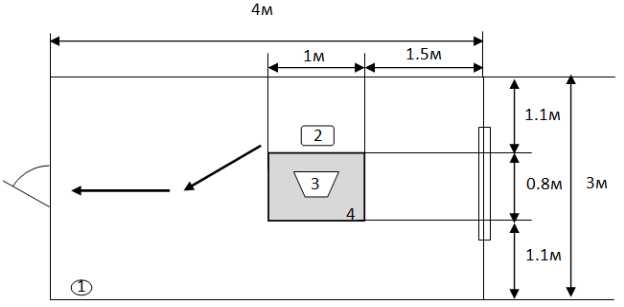
\includegraphics[scale=0.5]{graphics/workplace.png}
    \caption{Схема размещения рабочего места и план эвакуации}
    \label{fig:workplace}
\end{figure}

Обозначения для рисунка \ref{fig:workplace} :

\begin{enumerate}
    \item -- Огнетушитель ОУ-2;
    \item -- Стул;
    \item -- ПК;
    \item -- Стол.
\end{enumerate}

Для нормализации искусственного освещения рабочих зон необходима его реконструкция. Таким образом,
необходимо произвести выбор типа светильников и расчет их размещения в данном помещении.

Для искусственного освещения офиса рекомендуется использовать люминесцентные лампы, у которых большая световая отдача,
малая яркость светящейся поверхности, близкий к естественному спектральный состав излучения. Требуемая освещенность --
300 лк согласно ДБН В.2.5-28-2006.

Для данного типа помещений применяют потолочные светильника типа ЛВО 4Х18, имеющие следующие габариты 595Х595Х72мм.
В указанных светильниках применяются ЛЛ, в которых Фл = 1150лм.

Расчет освещенности производится методом коэффициента использования светового потока [1].
Расчет сводится к определению числа рядов светильников выбранного типа и числа светильников в ряду.

Расчетным методом является:

\begin{equation}\label{eq:main}
    N = \dfrac{E_{\text{н}} \times K_{\text{з}} \times S \times z}{n \times \text{Ф}_{\text{св}} \times \eta \times g}
\end{equation}
Где: 
\begin{itemize}
    \item $E_{\text{н}}$ - нормируемая минимальная освещенность, $E_{\text{н}}$ = 300 лк;
    \item $K_{\text{з}}$ - коэффициент запаса, учитывающий запыление светильников и износ источников света в процессе эксплуатации;
    \item S - площадь пола помещения, ${\text{м}}^2$; 
    \item z - коэффициент неравномерности освещения;
    \item n - число рядов светильников, определяемое из условия наивыгоднейшего соотношения $x = L \slash h$ (x = 1.4)
         (L - расстояние между рядами светильников(м); h -- высота подвеса светильников над рабочей поверхностю(м));
    \item g - коэффициент затенения (при отсутствии затенения g = 1); 
    \item $\eta$ - коэффициент использования светового потока; 
    \item ${\text{Ф}}_{\text{св}}$ - световой поток, излучаемый светильником, лм; 
\end{itemize}

При условии чистки светильников не реже двух раз в месяц $K_{\text{з}} = 1.4$. 
Для люминесцентных ламп z = 1.1. Коэффициент использования светового потока $\eta$ зависит от типа светильников,
коэффициентов отражения светового потока от стен $r{\text{c}}$, потолка $r{\text{п}}$ и пола $r{\text{пола}}$,
а также индекса помещения i:

\begin{equation}\label{eq:index}
    i = \dfrac{A \times B}{h \times (A + B)}
\end{equation}
Где:
\begin{itemize}
    \item A -- длина помещения;
    \item B -- ширина помещения;
    \item h -- высота подвеса светильников над рабочей поверхностью, м.
\end{itemize}

Высота подвеса светильников над рабочей поверхностью:

\begin{equation}\label{eq:high}
    h = H - H_{\text{рз}} - H_{\text{св}}
\end{equation}
Где:
\begin{itemize}
    \item H -- высота помещения, м;
    \item $H_{\text{рз}}$ -- высота рабочей поверхности над полом, $H_{\text{рз}}$ = 0.8 м;
    \item $H_{\text{св}}$ -- высота свеса светильника, $H_{\text{св}}$ = 0.4 м.
\end{itemize}

Расстояние между стенами и крайними рядами светильников рассчитывается следующим образом:

\begin{equation}\label{eq:length}
    l = (0.3 \ldots 0.5) \times L = 0.3 \times L
\end{equation}
Принимаем $r{\text{c}}$ = 50\%, $r{\text{п}}$ = 70\%,  $r{\text{пола}}$ = 10\% для данного помещения.
Подставим данные в формулы (1.1-1.4) и получим следующие результаты:
\[
    h = 2.5 - 0.8 - 0.4 = 1.3 (\text{м});
\]
\[
    L = 1.4 \times 1.3 = 1.82 (\text{м});
\]
\[
    l = 0.3 \times 1.82 \approx 0.5 (\text{м});
\]
\[
    n = \dfrac {1.82}{1.4} \approx 2;
\]
\[
    i = \dfrac {12}{1.3 \times 7} \approx 1.3;
\]
\[
    \eta = 0.48
\]

Поток, излучаемый светильником: ${\text{Ф}}_{\text{св}} = 4 \times 1150 = 4600$ лм.

По приведенной выше формуле \eqref{eq:main} определяем количество светильников в ряду:
\[
    N = 300 \times 1.4 \times 12 \times {\dfrac{1.2}{2}} \times 4600 \times 0.48 \times 1 = 1 (\text{шт})
\]
Таким образом, согласно расчетам для обеспечения оптимального уровня освещенности необходимо 2 ряда светильников по
одному в каждом ряде. Схема расположения светильников изображена на рисунке \ref{fig:torch}.

\begin{figure}[!ht]
    \centering
    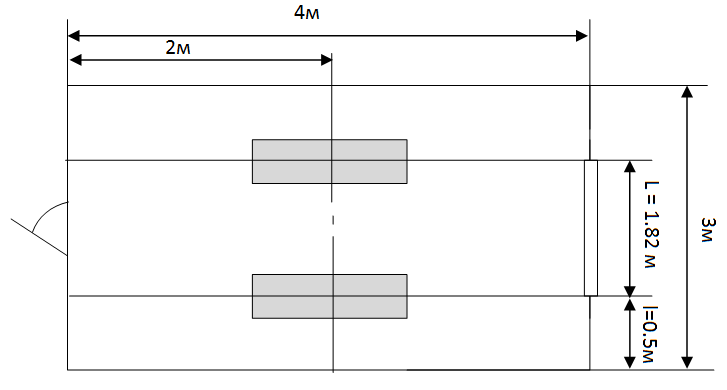
\includegraphics[scale=0.4]{graphics/torch.png}
    \caption{Схема расположения светильников}
    \label{fig:torch}
\end{figure}

\subsection{Безопасность в чрезвычайных ситуациях}

Согласно НАПБ Б.03.002-2007 помещение офиса относится к категории B,
так как в нем находятся горючие вещества и материалы. 

По пожароопасности помещение офиса относится к классу П-IIа в соответствии с НПАОП 40.1-1.21-98, 
так как в помещении находятся твердые горючие вещества (системный блок, монитор). В офисе присутствуют 
вещества и материалы, которые могут гореть (бумага, пластмасса, паркет). Данное помещение по степени огнестойкости,
согласно с ДБНВ.1.1.7-2002, относится к I степени огнестойкости. 

Причинами воспламенения в помещении могут служить: искрение в коммутационном оборудовании, 
замыкания в электрической сети, нарушение правил пожарной безопасности. 

Для предупреждения пожара необходимо проводить ряд технических и организационных мероприятий в соответствии 
с ГОСТ 12.1.004 – 91.

В системе предотвращения пожара предусмотрено:

\begin{itemize}
    \item коммутация проводов выполнена разъемами;
    \item сечение проводов выбрано в соответствии с максимальным током нагрузки;
    \item использование максимально негорючих веществ и материалов.
\end{itemize}

Помещение оборудовано двумя огнетушителем ВВК-1,4 согласно НАПБ Б.03.001-2004  из расчета один огнетушитель на 3 ПЭВМ,
но не меньше двух в помещении, а также электрической пожарной сигнализацией согласно НАПБ Б.03.001-2004 из расчета 
не менее двух в помещении, состоящей из комбинированных тепловых и дымовых извещателей типа КИ–1 в количестве 2 шт.,
температура срабатывания которых составляет 50–80$^{\circ}\mathrm{C}$.

Для успешной эвакуации персонала при пожаре размеры дверей рабочего помещения имеют следующие габариты: 
ширина  – 1,5 м, высота -  2,0 м, а ширина коридора - 1,8 м.  При возникновении пожара осуществляется эвакуация людей, 
находящихся в помещении, в соответствии с планом эвакуации (рисунок \ref{fig:workplace}).

